% Copyright (c) 2011, Yifan Peng <yfpeng@udel.edu>
% All rights reserved.
% 
% Redistribution and use in source and binary forms, with or without
% modification, are permitted provided that the following conditions are met:
% 1. Redistributions of source code must retain the above copyright
%    notice, this list of conditions and the following disclaimer.
% 2. Redistributions in binary form must reproduce the above copyright
%    notice, this list of conditions and the following disclaimer in the
%    documentation and/or other materials provided with the distribution.
% 3. All advertising materials mentioning features or use of this software
%    must display the following acknowledgement:
%    This product includes software developed by the <organization>.
% 4. Neither the name of the <organization> nor the
%    names of its contributors may be used to endorse or promote products
%    derived from this software without specific prior written permission.
% 
% THIS SOFTWARE IS PROVIDED BY <COPYRIGHT HOLDER> ''AS IS'' AND ANY
% EXPRESS OR IMPLIED WARRANTIES, INCLUDING, BUT NOT LIMITED TO, THE IMPLIED
% WARRANTIES OF MERCHANTABILITY AND FITNESS FOR A PARTICULAR PURPOSE ARE
% DISCLAIMED. IN NO EVENT SHALL <COPYRIGHT HOLDER> BE LIABLE FOR ANY
% DIRECT, INDIRECT, INCIDENTAL, SPECIAL, EXEMPLARY, OR CONSEQUENTIAL DAMAGES
% (INCLUDING, BUT NOT LIMITED TO, PROCUREMENT OF SUBSTITUTE GOODS OR SERVICES;
% LOSS OF USE, DATA, OR PROFITS; OR BUSINESS INTERRUPTION) HOWEVER CAUSED AND
% ON ANY THEORY OF LIABILITY, WHETHER IN CONTRACT, STRICT LIABILITY, OR TORT
% (INCLUDING NEGLIGENCE OR OTHERWISE) ARISING IN ANY WAY OUT OF THE USE OF THIS
% SOFTWARE, EVEN IF ADVISED OF THE POSSIBILITY OF SUCH DAMAGE.
\PassOptionsToPackage{rgb}{xcolor}
\documentclass{beamer}

\mode<presentation>
\usetheme{Udel}

\usepackage{alltt}
\usepackage[english]{babel}
\usepackage{pgf}
\usepackage{amssymb}
\usepackage{amsmath}
\usepackage{tikz}
\usepackage{xmpmulti}
\usepackage{ulem}
%\usepackage{beamerprosper}
\usepackage{calc}
\usepackage{multirow}
\usepackage{colortbl}
\usepackage{tabularx}
\usepackage{mathptmx}
\usepackage{helvet}


\DeclareGraphicsRule{*}{mps}{*}{}
\DeclareMathOperator*{\argmax}{\arg\max}

\graphicspath{{images/}}
%\setbeamerfont{title}{
%	size=\Large,
%	series=\bfseries,
%	shape=\scshape,
%	family=\rmfamily
%}

\usetikzlibrary{%
  arrows,%
  automata,%
  calc,%
  trees,%
  positioning,%
  chains,%
  shapes,%
  shapes.arrows,%
  shapes.geometric,%
  shapes.misc,% wg. rounded rectangle
  shapes.symbols,%
  decorations.pathreplacing,%
  decorations.pathmorphing,% /pgf/decoration/random steps | erste Graphik
  matrix,%
  scopes,%
  shadows%
 }

%\includeonlyframes{cur}


\title{Beamer Theme with \\University of Delaware Logo (v3)}
\author[Yifan Peng]{Yifan Peng}
\institute[Computer \& Information Sciences]{Computer \& Information
Sciences}
\date[today]{\today}

\pgfdeclarelayer{background}
\pgfdeclarelayer{foreground}
\pgfsetlayers{background,main,foreground}


\begin{document}

\begin{frame}[plain]
    \titlepage
\end{frame}

\begin{frame}
\frametitle{Outline} \tableofcontents[hideallsubsections]
\end{frame}

\section{UD Colors}

\begin{frame}
\frametitle{UD Colors}
\begin{exampleblock}{University Colors}
\begin{itemize}
  \item Udel blue: \textcolor{udelblue}{RGB: 0, 83, 159}
  \item Udel dark blue: \textcolor{udeldarkblue}{RGB: 0, 38, 99}
  \item Udel yellow: \textcolor{udelyellow}{RGB: 255, 210, 0}
\end{itemize}
\end{exampleblock}
\end{frame}

\section{UD Primary Logo}

\begin{frame}
\frametitle{UD Primary Logo}
\begin{figure}
	
\includegraphics[width=.5\textwidth]{UDPrimaryLogo2945.pdf}
\end{figure}
\end{frame}

\section{Diagram}

\begin{frame}[fragile] 
\frametitle{Graphitemize}
\begin{center}

\begin{tikzpicture}
\footnotesize

\definecolor{color1}{RGB}{0,84,150}
\definecolor{color2}{RGB}{202,108,24}

% center, radius, text 
\newcommand{\primary}[3]{
  \draw[align=center,thick] #1 node{#3};
  \begin{pgfonlayer}{background}
    \draw[ultra thick,
	      draw=none,
	      shade=ball,
          circular drop shadow,
	      fill opacity=.7,
          ball color=color2!60!black] #1 circle (#2);
  \end{pgfonlayer}
}

\newcommand{\secondary}[3]{
  \draw[align=center] #1 node{#3};
  \begin{pgfonlayer}{background}
    \draw[ultra thick,
	      draw=white,
	      fill opacity=.7,
          fill=color1!40] #1 circle (#2);
  \end{pgfonlayer}
}

\tikzstyle{type}=[
     ultra thick,
     draw=white,
     fill opacity=.7,
     fill=color1,
]


\draw[align=center](0:0cm) node{iSimp};
\begin{pgfonlayer}{background}
  \draw[type,fill=gray!40,fill opacity=.7] (0:0cm) circle (2cm);
\end{pgfonlayer}

\primary{(0:3cm)}{1.5cm}{Coordinations}
\primary{(70:2.9cm)}{1.3cm}{Relative\\clauses}
\primary{(300:2.3cm)}{0.48cm}{Appositions}

\secondary{(250:2.3cm)}{0.40cm}{Subordinate\\clauses}
\secondary{(200:2.2cm)}{1.08cm}{Introductory\\phrases}
\secondary{(135:2.6cm)}{1.29cm}{Parenthesised\\elements}

\end{tikzpicture}
\end{center}
\end{frame}

\begin{frame}[fragile] 
\frametitle{Linear Flow}
\begin{tikzpicture}

\definecolor{color1}{RGB}{255,187,0}
\definecolor{color2}{RGB}{150,211,51}
\definecolor{color3}{RGB}{0,195,201}

% center point, color left text, right text
\newcommand{\oneblock}[4]{
  \draw #1 node {
  \begin{tikzpicture}[node distance=0em]
  \node[draw=#2,
        rounded corners,
        line width=4pt,
        inner sep=4pt,
        text justified,
        text width=.7\textwidth,
        minimum height=4em](a) {#4};
  \draw[fill=#2,draw=none]
        let \p1=(a.north west), 
            \p2=(a.south west),
            \p3=(\x1+5pt,\y1),
            \p4=(\x2+5pt,\y2) in
        (\p3)--(\x3-3em,\y3-1.5em)--(\x3-6em,\y3)
        --(\x4-6em,\y4)--(\x4-3em,\y4-1.5em)--(\p4)--cycle;
  \node[right =of a.west,
        xshift=-3em+5pt, 
        yshift=-1em, 
        anchor=center, 
        align=center] {#3};
  \end{tikzpicture}
  };
}

\newcommand*{\entity}[1]{\textcolor{blue}{#1}}
\oneblock{(0em,0em)}{color1}{Training set}{
    $\bullet$ ~ \entity{PKC} \uwave{phosphorylates} \entity{GAP-43} on serine 41.\\
    $\bullet$ ~ \entity{JNK} \uwave{phosphorylates} \entity{BAD} at threonine 201.\\
    $\bullet$ ~ $\cdots$
}
\oneblock{(0em,-5em)}{color2}{Learned\\rules}{
	\entity{A} \uwave{phosphorylates} \entity{B}, \\
    when \entity{A} and \entity{B} are proteins
}
\oneblock{(0em,-10em)}{color3}{New Data}{
	It was suggested that \entity{Yak1} \uwave{phosphorylates} \entity{Crf1} to promote its nuclear entry.
}
\end{tikzpicture}
\end{frame}

\begin{frame}[label=bar,fragile]
\frametitle{Horizontal Bar Chart}
\begin{figure}
\vspace*{-2em}
\centering
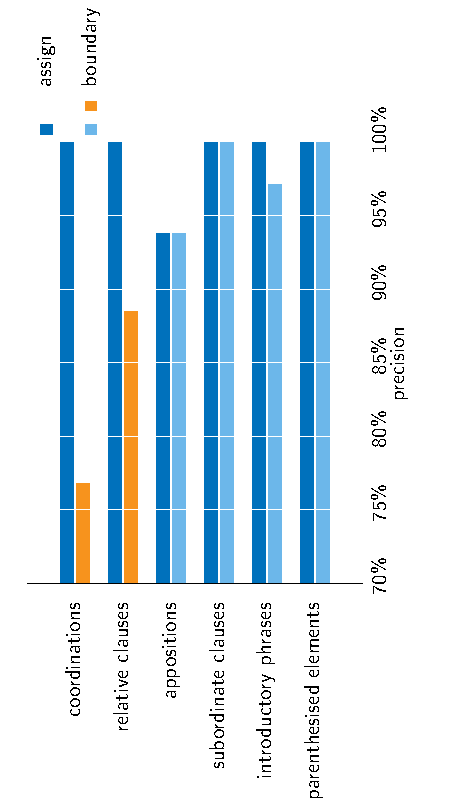
\includegraphics[height=\textwidth,angle=-90]{fvaluemodify.pdf}
\end{figure}
\end{frame}

\begin{frame}[label=bar2,fragile]
\frametitle{Horizontal Bar Chart}
\begin{figure}
\centering
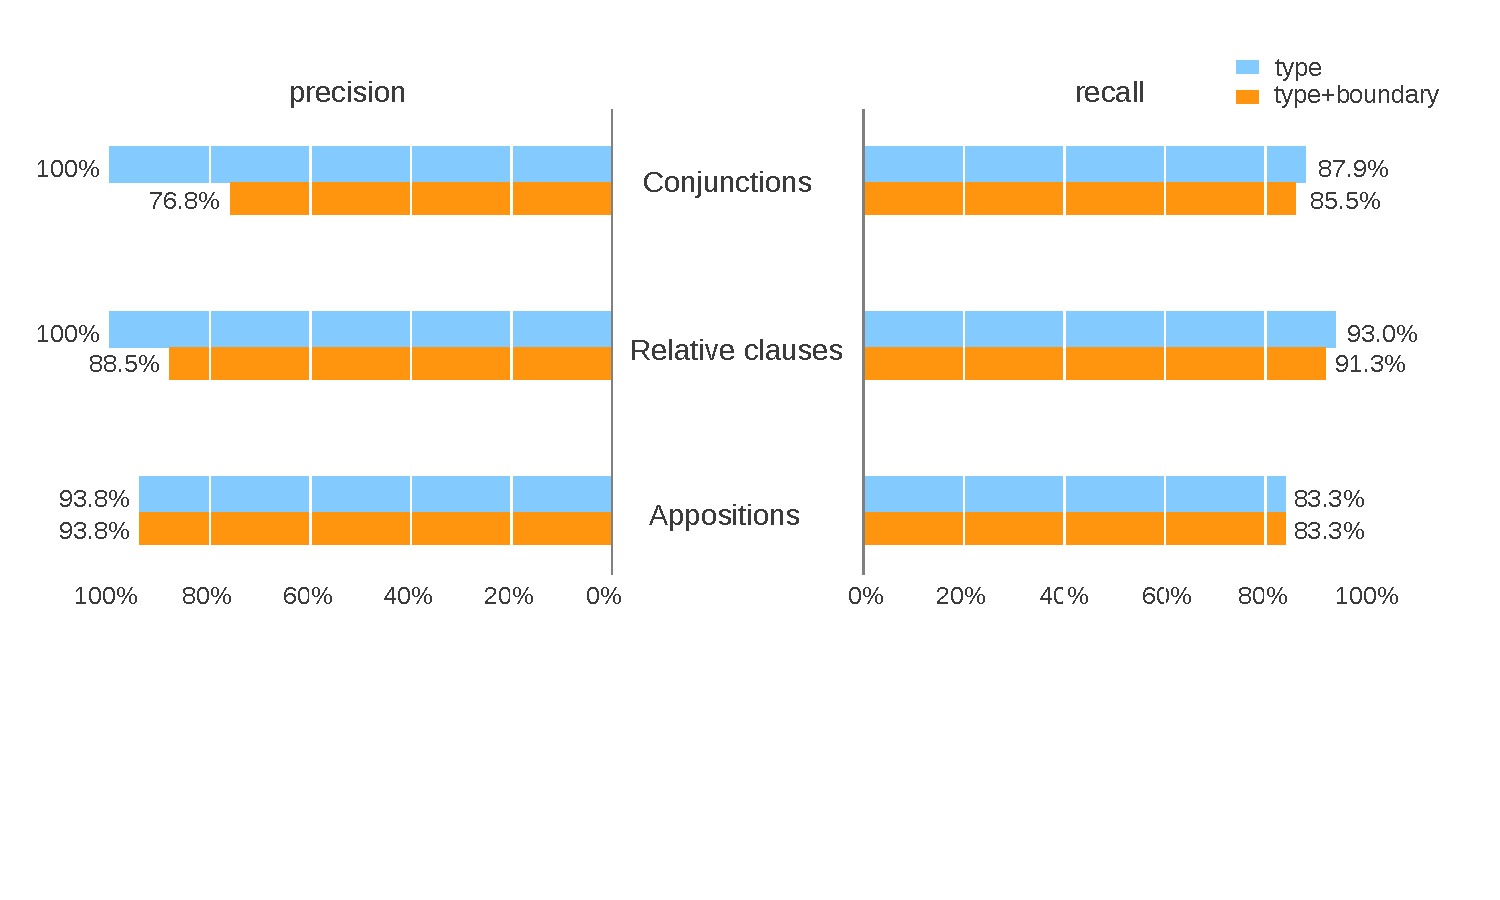
\includegraphics[width=\textwidth]{precision7.pdf}
\end{figure}
\end{frame}

\begin{frame}[label=color,fragile]
  \frametitle{Color in tables}
  \begin{table}
  \begin{tabular}{l|l}
    \hline
    \rowcolor{udelblue}\color{white}xxxxxxxxxxxxxxxxxx & \color{white}xxxxxxxxxxxxxxxxxxx \\
    \hline
    yyyyyyyyyyyyyy & yyyyyyyyyyy \\
    zzzzzzzzz & zzzzzzzzzz \\
    zzzzzzzzz & zzzzzzzzzz \\
    \hline
  \end{tabular}
  \end{table}
\end{frame}

\begin{frame}[label=colorwheel,fragile]
  \frametitle{Colorwheel}
\begin{center}
\vspace{-1em}
\begin{tikzpicture}
\footnotesize
% Create the background in the circle, by drawing several slices
% each with a constant color given by the angle (which is converted
% to a color usin the hue, saturation and brightness color space).
\foreach \x in {0,0.0416,...,1} {
	\definecolor{currentcolor}{hsb}{\x, 1, 1}
	\draw[draw=none, fill=currentcolor]
		(-360*\x+88-7.5:0) -- (-360*\x+88-7.5:2.7)
		arc (-360*\x+88-7.5:-360*\x+88+7.5:2.7) -- cycle;
}
% Draw a circle with markings along the perimeter, indicating which angles
% the hue function connects to certain colors.
\draw (0, 0) circle (2.7);
\foreach \x  in {0, 30, ..., 330}
	\draw (-\x+90:2.8) -- (-\x+90:2.7) (-\x+90:3); % node {$\x^\circ$};

% Add labels with names of the primary and secondary colors.
\foreach \x/\text in {%
	0/\begin{tabular}{c}Red\\255-0-0\end{tabular}, 
	60/\begin{tabular}{c}Yellow\\255-255-0\end{tabular}, 
	120/\begin{tabular}{c}Green\\0-255-0\end{tabular}, 
	180/\begin{tabular}{c}Cyan\\0-255-255\end{tabular}, 
	240/\begin{tabular}{c}Blue\\0-0-255\end{tabular}, 
	300/\begin{tabular}{c}Magenta\\255-0-255\end{tabular},
%
	30/\begin{tabular}{c}Orange\\255-125-0\end{tabular}, 
	90/\begin{tabular}{c}Spring Green\\125-255-0\end{tabular}, 
	150/\begin{tabular}{c}Turquoise\\0-255-125\end{tabular}, 
	210/\begin{tabular}{c}Ocean\\0-125-255\end{tabular}, 
	270/\begin{tabular}{c}Violet\\125-0-255\end{tabular}, 
	330/\begin{tabular}{c}Raspberry\\255-0-125\end{tabular},
	}
	\draw (-\x+90:3.3) node {\text};
\end{tikzpicture}
\end{center}
\end{frame}

\begin{frame}
	\frametitle{\;}
\begin{center}
\huge Q \& A \vspace{1em}
\end{center}
\end{frame}

\end{document}
